\documentclass[11pt]{article}
\usepackage[utf8]{inputenc}
\usepackage[spanish]{babel}
\usepackage{amsmath,amssymb,amsthm}
\usepackage{graphicx}

\usepackage{hyperref}

\title{\huge{\textbf{Análisis asintótico de algoritmos}}}
\author{\large{\textbf{Sergio Revilla Velasco}}}

\date{}

\renewcommand{\P}{\ensuremath{\textup{\textbf{P}}}}

\newcommand{\E}{\ensuremath{\textup{\textbf{E}}}}

\begin{document}
\maketitle


\begin{abstract}
%\noindent
El objetivo de esta práctica es estudiar la complejidad asint\'otica de los algoritmos de selecci\'on(selection-sort), inserci\'on(insertion-sort), burbuja (bubble-sort), ordenaci\'on r\'apida (quick-sort) y ordenaci\'on por mezcla (merge-sort) por medio de un programa escrito en C++
\end{abstract}

\tableofcontents{}
%\setlength{\parindent}{0pt}
\newpage

\section{Instrucciones de compilación y dependencias}
\begin{enumerate}
	\item Dependencias
		\begin{itemize}
			\item Windows: MinGW  \url{http://www.mingw.org}
			\item Linux: GCC Compiler Collection  \url{http://gcc.gnu.org}
			\item Mac Os X: Xcode Tools con utilidades de línea de comando instaladas  							\url{https://developer.apple.com/xcode/}
			\item GnuPlot: usado para generar las gr\'aficas desde archivos de texto 								\url{http://www.gnuplot.info}
		\end{itemize}
	\item Instrucciones de compilaci\'on
			\begin{itemize}
			\item Compilar el archivo \emph{main.cpp} contenido en la carpeta \emph{/src}
			\item El programa generar\'a archivos \emph{txt} separado por l\'ineas, con el tamaño 				del problema y el tiempo empleado en la ordenaci\'on expresado en milisegundos 					\emph{(ms)}.  
			\item Ejecutar desde la consola el comando \emph{gnuplot script.gnuplot} desde el 					mismo directorio donde se generaron los archivos de datos.
			\item El script generar\'a archivos \emph{png} con las gr\'aficas.
			\end{itemize}
\end{enumerate}

\newpage
\section{Método de obtención de tiempos y gráficas}
	\begin{enumerate}
		\item El programa preguntará por el tamaño del problema (la longitud del array)
		\item También podemos elegir el mayor entero a generar (un entero puede tener un valor 				máximo de $32767$ )
		\item El programa preguntará por el salto \emph{(gap)} entre iteraciones.  En primera instancia se genera un array con números aleatorios que sirve como base para las ordenaciones.  De esta manera las copias del array original se hacen del tamaño que corresponde a la iteración, en lugar de hacer copias con el tamaño original del problema y así evitar problemas de memoria para tamaños del problema muy grandes $(n > 20000)$
\end{enumerate}


\newpage
\section{Gráficas de tiempos obtenidas}


%Gráfica de ordenación por inserción
\begin{figure}
  \centering
    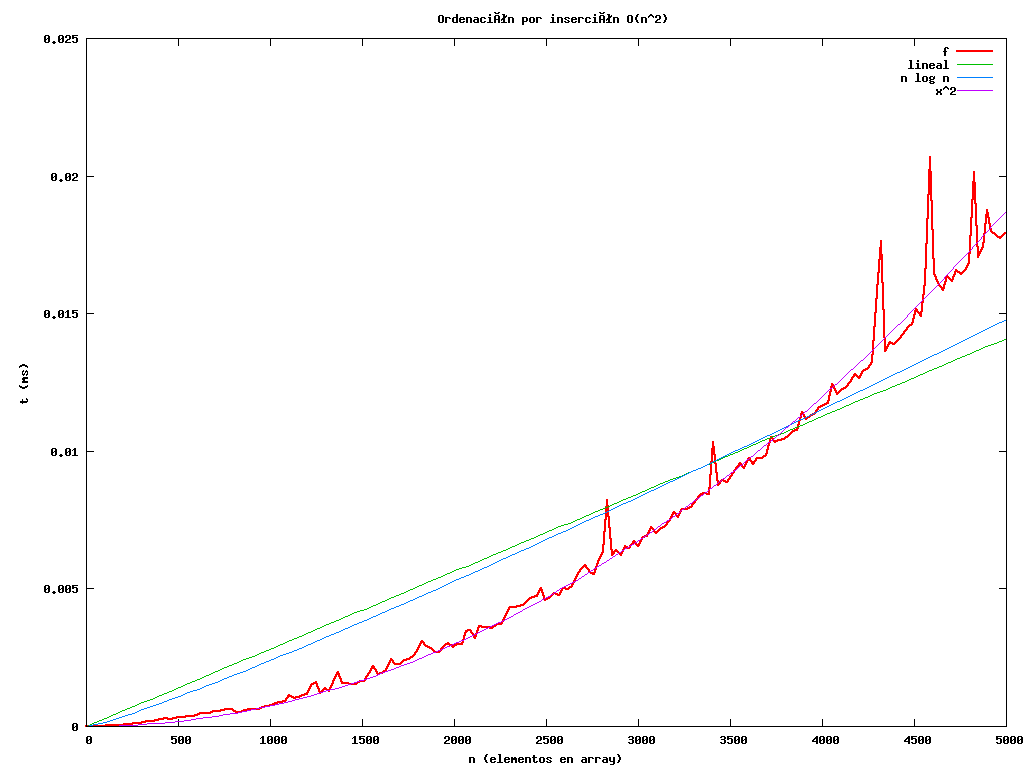
\includegraphics[width=1.0\textwidth]{insertion-sort.png}
  \caption{Ordenación por inserción}
  \label{fig:insertion}
\end{figure}

%Gráfica de ordenación por selección
\begin{figure}
  \centering
    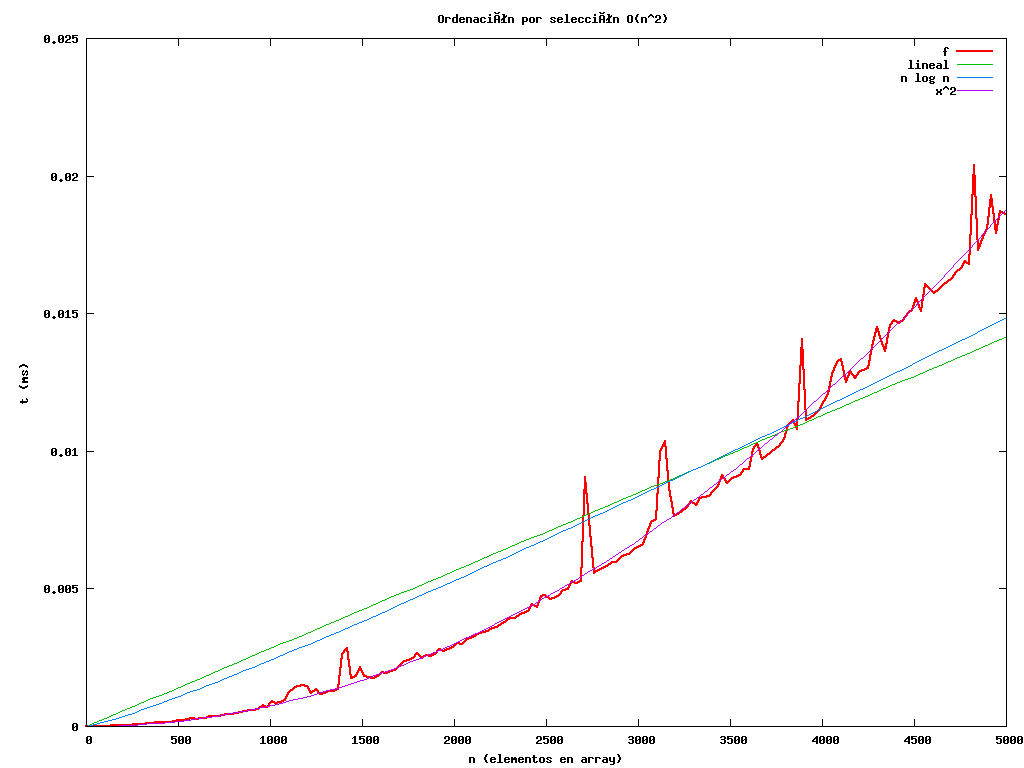
\includegraphics[width=1.0\textwidth]{selection-sort.png}
  \caption{Ordenación por selección}
  \label{fig:selection}
\end{figure}

%Gráfica de ordenación por burbuja
\begin{figure}
  \centering
    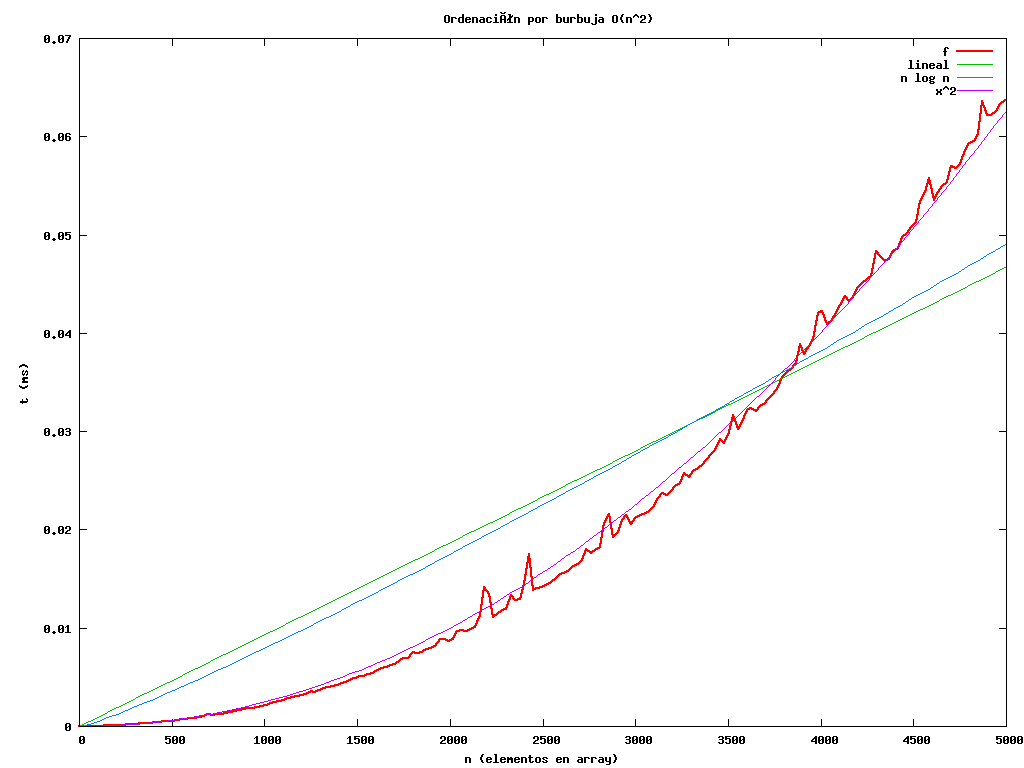
\includegraphics[width=1.0\textwidth]{bubble-sort.png}
  \caption{Ordenación por burbuja}
  \label{fig:bubble}
\end{figure}

%Gráfica de ordenación rápida
\begin{figure}
  \centering
    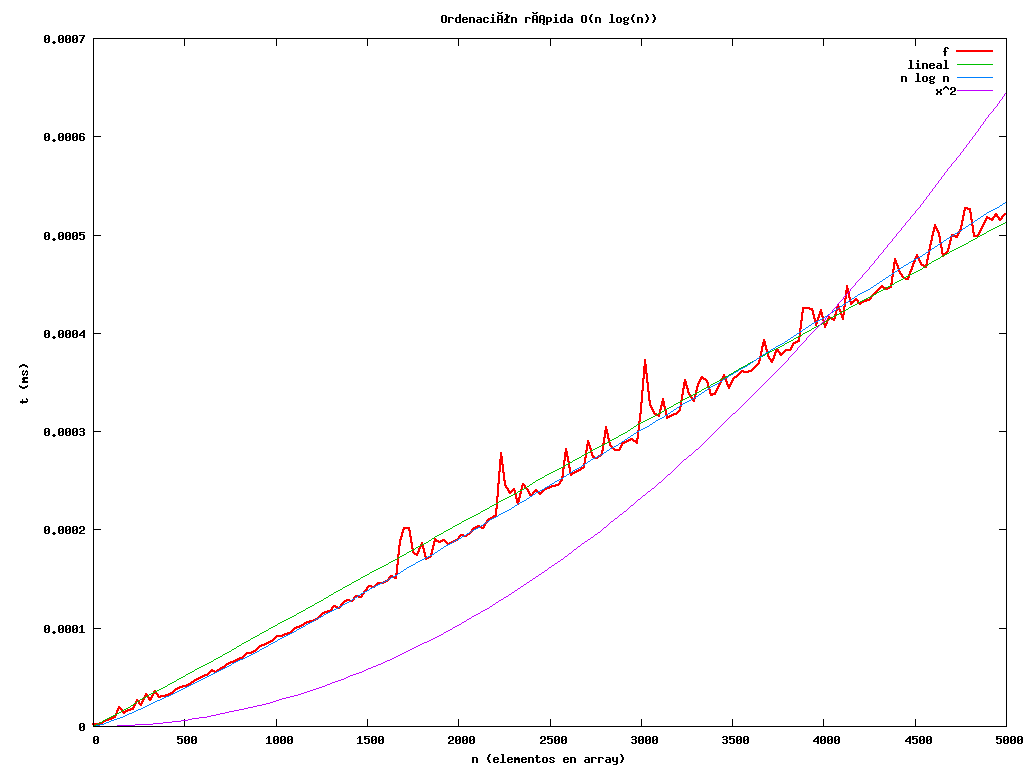
\includegraphics[width=1.0\textwidth]{quick-sort.png}
  \caption{Ordenación rápida}
  \label{fig:quick}
\end{figure}

\newpage
\section{Análisis de las gráficas}




\newpage
\section{Comentarios adicionales}

\end{document}